\documentclass[crop, tikz]{standalone}

\definecolor{nonphotoblue}{HTML}{A4DDED}
\usetikzlibrary{decorations.pathmorphing,patterns}
\begin{document}
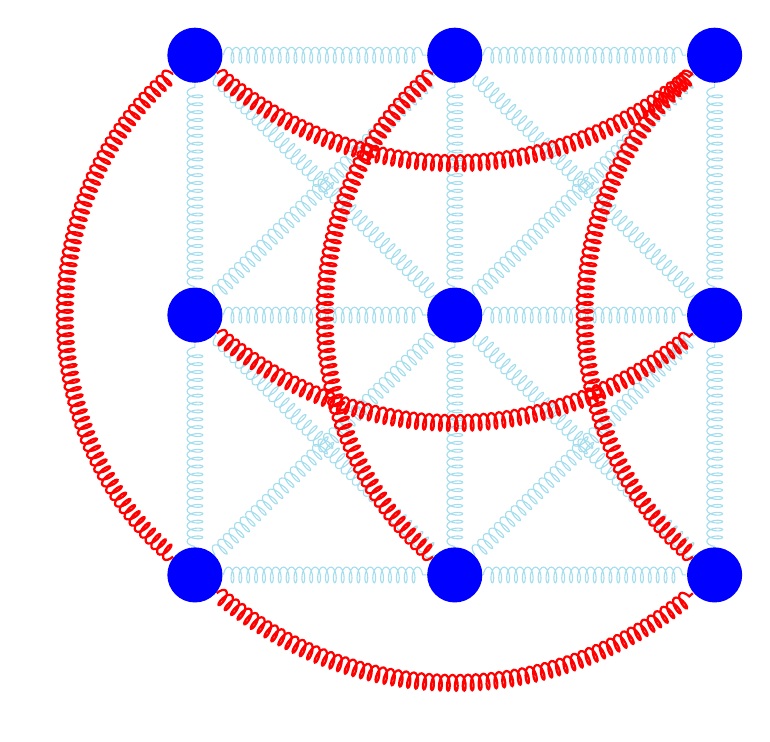
\begin{tikzpicture}[draw=nonphotoblue, text=nonphotoblue, scale=1.65, transform shape, decoration={aspect=0.4, segment length=1mm, amplitude=1mm,coil}]
\node[circle,fill=blue,inner sep=1.5mm] (a11) at (0, 0) {};
\node[circle,fill=blue,inner sep=1.5mm] (a12) at (2, 0) {};
\node[circle,fill=blue,inner sep=1.5mm] (a13) at (4, 0) {};

\node[circle,fill=blue,inner sep=1.5mm] (a21) at (0, 2) {};
\node[circle,fill=blue,inner sep=1.5mm] (a22) at (2, 2) {};
\node[circle,fill=blue,inner sep=1.5mm] (a23) at (4, 2) {};

\node[circle,fill=blue,inner sep=1.5mm] (a31) at (0, 4) {};
\node[circle,fill=blue,inner sep=1.5mm] (a32) at (2, 4) {};
\node[circle,fill=blue,inner sep=1.5mm] (a33) at (4, 4) {};

% Horizontal springs
\draw[decorate] (a11) -- (a12);
\draw[decorate] (a12) -- (a13);

\draw[decorate] (a21) -- (a22);
\draw[decorate] (a22) -- (a23);

\draw[decorate] (a31) -- (a32);
\draw[decorate] (a32) -- (a33);

% Vertical springs
\draw[decorate] (a11) -- (a21);
\draw[decorate] (a12) -- (a22);
\draw[decorate] (a13) -- (a23);

\draw[decorate] (a21) -- (a31);
\draw[decorate] (a22) -- (a32);
\draw[decorate] (a23) -- (a33);

% /-Diagonal springs
\draw[decorate] (a11) -- (a22);
\draw[decorate] (a12) -- (a23);
\draw[decorate] (a21) -- (a32);
\draw[decorate] (a22) -- (a33);

% \-Diagonal springs
\draw[decorate] (a12) -- (a21);
\draw[decorate] (a13) -- (a22);
\draw[decorate] (a22) -- (a31);
\draw[decorate] (a23) -- (a32);

% Horizontal Bending Springs
\draw[ decorate, red, thick] (a11) to[out=-40,in=220] (a13);
\draw[ decorate, red, thick] (a21) to[out=-40,in=220] (a23);
\draw[ decorate, red, thick] (a31) to[out=-40,in=220] (a33);

% Vertical Bending Springs
\draw[ decorate, red, thick] (a11) to[out=140,in=220] (a31);
\draw[ decorate, red, thick] (a12) to[out=140,in=220] (a32);
\draw[ decorate, red, thick] (a13) to[out=140,in=220] (a33);
\end{tikzpicture}
\end{document}

